%Getting Started
\section{Getting Started}
Die Inbetriebnahme unserer Implementation erfolgt sehr simpel über die entsprechende Funktion von Visual Studio, sollte man sich zum Import in die IDE entscheiden, oder über die beigefügte .exe Datei.
Es ist zu beachten, dass SimOS eine \textit{processes.txt} Datei entweder im Projektordner für Visual Studio oder im selben Ordner wie die .exe erwartet. Diese Datei dient als Liste von Prozessen, die von SimOS einzulesen und auszuführen sind.
Die processes.txt baut sich folgendermaßen auf: Man legt pro Zeile die Informationen zu einem Prozess fest, wobei die erste Zeile als Kommentar gewertet wird. Die Informationen müssen sich in der Reihenfolge OwnerID, start, duration, size, type in der Datei befinden.
Eine beispielhafte Datei würde etwa so aussehen: \\
\begin{figure}[!h]
    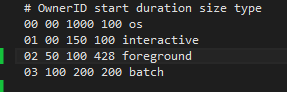
\includegraphics[scale=1]{img/processes}
    \caption{processes.txt}
\end{figure}

Die entsprechende Datei würde folgende Ausgaben generieren:\\
\begin{figure}[!h]
    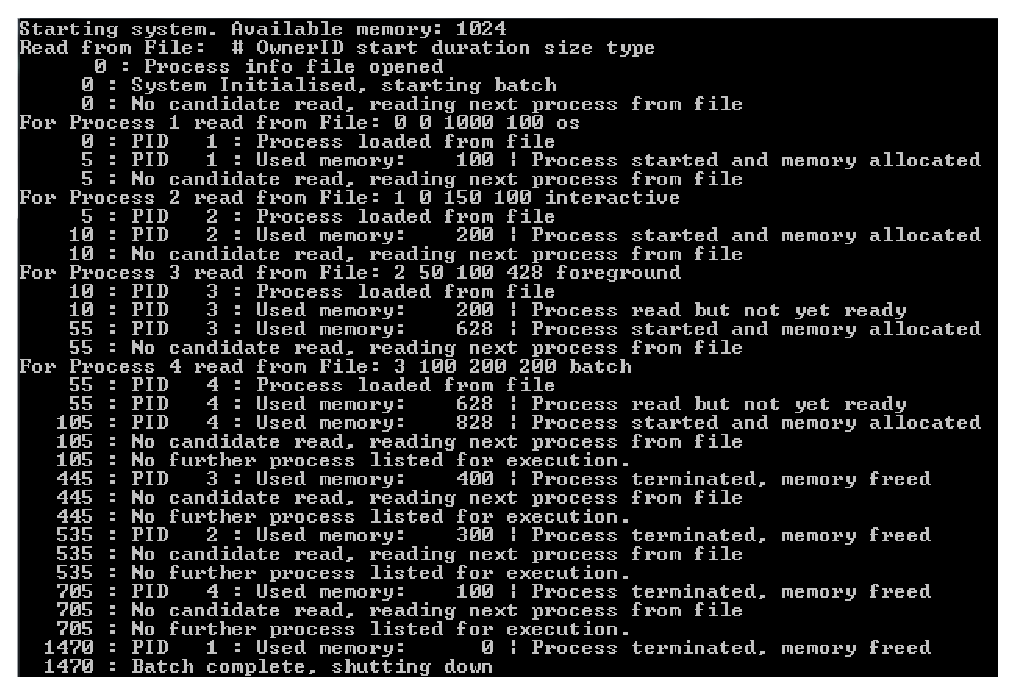
\includegraphics[scale=1]{img/output}
    \caption{Output für processes.txt}
\end{figure}
